\textbf{Цель работы:} практическое ознакомление с принципами записи и восстановление оптических голограмм, запись и восстановление голограммы по схеме Денисюка.

\textbf{Аппаратура:} полупроводниковый лазер, фотопластинка, проявитель, закрепитель, объект, фиксирующая рама, фонарь.

\section{Минимальные теоретические сведения}

Схема записи Денисюка (\autoref{fig:optical_scheme})~--- оптическая схема записи аналоговой отражающей голограммы во встречных пучках. Данная схема отличается простотой сборки и использования и состоит из полупроводникового лазера, имеющего малые размеры и дающего расходящийся пучок без применения линз, фотопластинки и объекта. В схеме опорный и предметный пучки падают на пластинку с разных сторон, формируя на ней дифракционную решетку с пространственно-периодическими слоями почернения. Получаемая аналоговая голограмма обладает спектральной селективностью и использует для восстановления длину волны видимого света, удовлетворяющую условию Вульфа-Брэгга. Благодаря этому изображение видно в обычном белом свете, что значительно упрощает процесс восстановления.

\begin{figure}[h]%
    \centering
    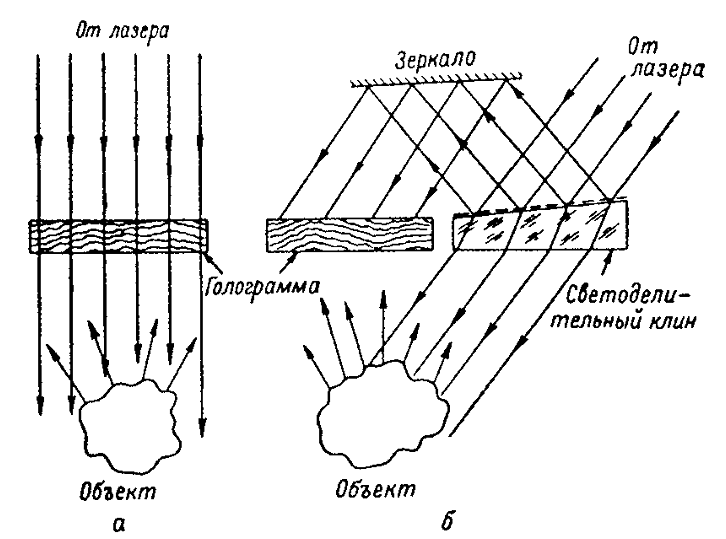
\includegraphics[width=0.8\textwidth]{optical_scheme}%
    \caption[]{Оптические схемы записи голограммы во встречных пучках}%
    \label{fig:optical_scheme}%
\end{figure}

Для записи голограммы Денисюка оптимально подходят непрозрачные объекты. Объект должен обладать достаточной прочностью всех деталей и элементов. Желательно, чтобы он был изготовлен из металла, фарфора или твердой керамики. Объекты из дерева, пластмассы, бумаги регистрировать гораздо сложнее, т.к. по время регистрации просиходит сдвиг отдельных деталей и элементов структуры этих объектов, что приводит к \enquote{размытию} интерференционной картины.

При регистрации голограммы необходимы устойчивые механические оптико-системы, защищенные от вибрации во время экспозиции фотопластинок, регистрирующих голограммы. Даже незначительное взаимное смещение элементов оптической системы, порядка долей длины световой волны источника света, приводит к размытию интерференционной картины на голограмме и к утрате записываемой на ней информации об объекте наблюдения. Поэтому оптическую схему необходимо собирать на специальном оптическом столе, либо использовать массивную плиту, расположенную, например, на накаченной автомобильной шине или ванне с песком. Большая масса необходима для того, чтобы сделать частоту собственных колебаний оптического стола много меньше частот колебаний здания.

В ходе эксперимента необходимо соблюдать полную тишину и обеспечить отсутствие вибраций.

\section{Анализ результатов}

В ходе эксперимента была записана голограмма объекта наблюдения \enquote{мышь} (\autoref{fig:mouse}) на фотопластинке. Результат восстановления изображения представлен на \autoref{fig:result}.

\begin{figure}[h]%
    \centering
    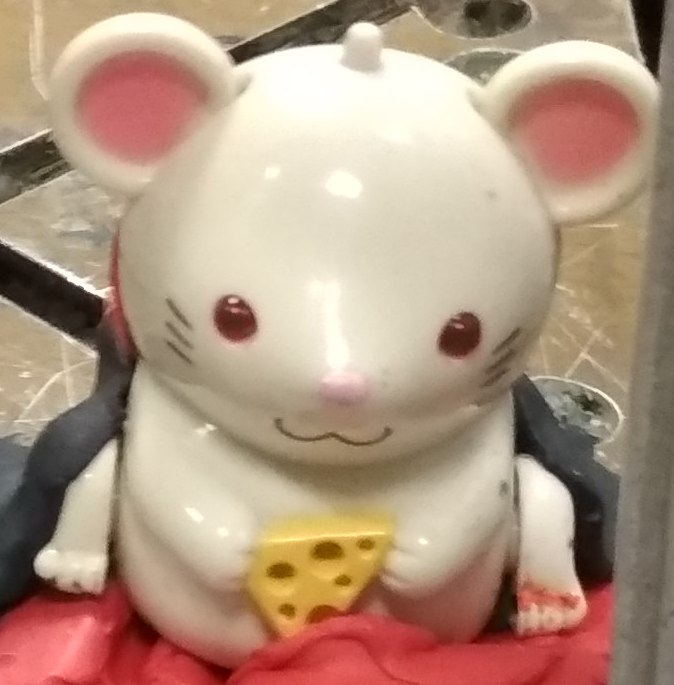
\includegraphics[width=0.8\textwidth]{mouse}%
    \caption[]{Объект наблюдения}%
    \label{fig:mouse}%
\end{figure}

\begin{figure}[h]%
    \centering
    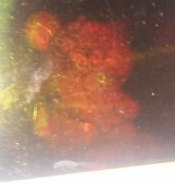
\includegraphics[width=0.8\textwidth]{result}%
    \caption[]{Результат восстановления}%
    \label{fig:result}%
\end{figure}

Изображение, формируемое при восстановлении голограммы кажется объемным. При повороте источника восстанавливающего светового пучка относительно плоскости пластинки восстановленное изображение поворачивается, что свидетельствует о наличии на фотопластинке информации не только об амплитуде, но и о фазовом распределении записанного изображения, т.е. в некоторой степени об успешной записи голограммы.

Голограмма качественно восстанавливается любым источником белого света.

\section{Выводы}

  В ходе работы была записана и впоследствии восстановлена голограмма по схеме Денисюка. Записанное изображение восстанавливается любым источником белого света в \enquote{объемную} картину.